% Architecture view of the smoked AC-Gömb prototype (one shared HSiKAN trunk -> actor + critic heads).
% Numbers are from the 2026-06-22 Galambos smoke: N=6 link vertices, feat=8, hidden=64, L=2, |a|=4;
% shared trunk = 14,537 params vs 28,745 with two separate backbones.
\documentclass[border=8pt]{standalone}
\usepackage{amsmath}
\usepackage{amssymb}
\usepackage{xcolor}
\usepackage{tikz}
\usetikzlibrary{arrows.meta,positioning,fit,backgrounds,calc}
\tikzset{
  io/.style   ={draw, rounded corners, align=center, font=\small, fill=gray!8, minimum height=10mm},
  lyr/.style  ={draw, rounded corners, align=center, font=\small, fill=blue!6, minimum height=12mm, minimum width=26mm},
  head/.style ={draw, rounded corners, align=center, font=\small, fill=orange!12, minimum height=11mm, very thick},
  oport/.style  ={draw, rounded corners, align=center, font=\small, fill=green!8, minimum height=10mm},
  vtx/.style  ={circle, draw, minimum size=4.5mm, inner sep=0pt, font=\tiny, fill=blue!10},
  arr/.style  ={-{Stealth[length=2.4mm]}, thick},
  epos/.style ={-{Stealth[length=1.8mm]}, semithick, draw=green!55!black},
  eneg/.style ={-{Stealth[length=1.8mm]}, semithick, draw=red!60, dashed},
}
\begin{document}
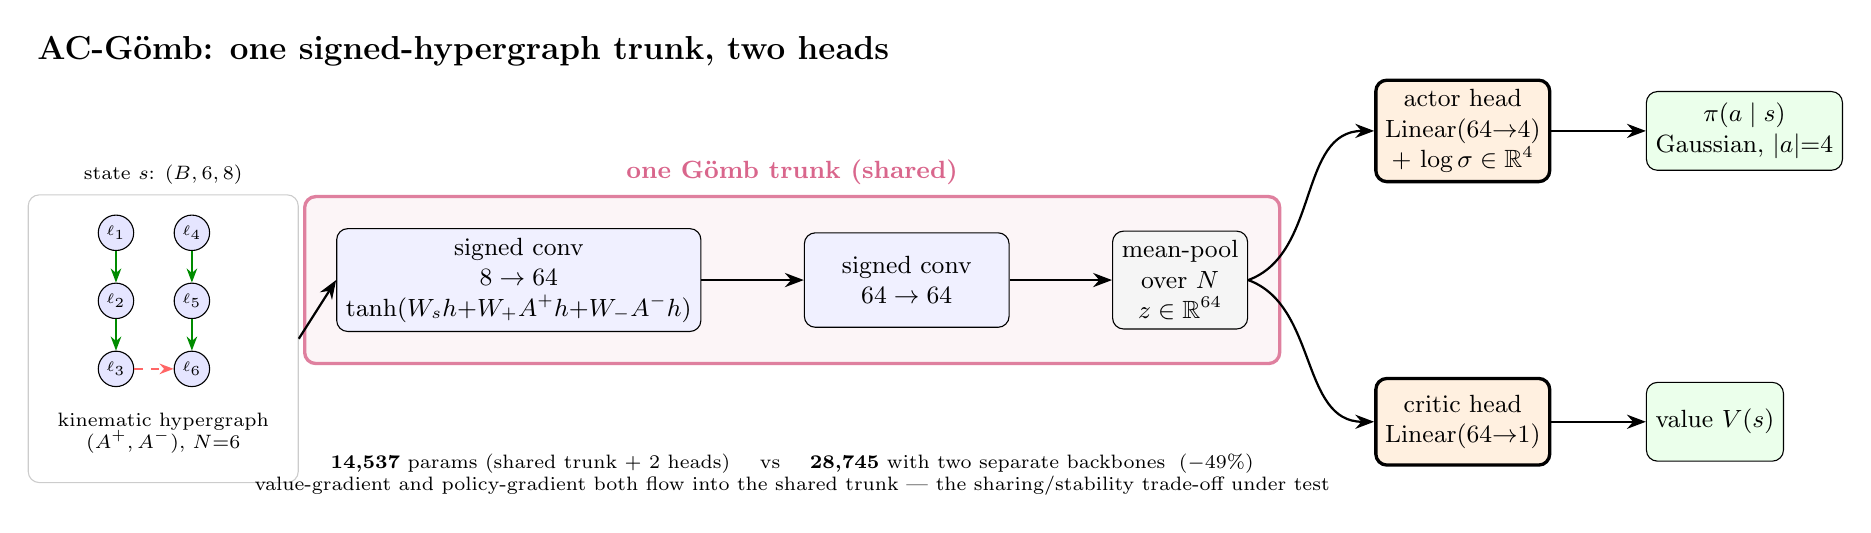
\begin{tikzpicture}[node distance=9mm and 13mm]

  % ---- input: per-vertex state on the kinematic hypergraph ----
  \node[vtx] (a1) {$\ell_1$};
  \node[vtx, below=4mm of a1] (a2) {$\ell_2$};
  \node[vtx, below=4mm of a2] (a3) {$\ell_3$};
  \node[vtx, right=5mm of a1] (a4) {$\ell_4$};
  \node[vtx, below=4mm of a4] (a5) {$\ell_5$};
  \node[vtx, below=4mm of a5] (a6) {$\ell_6$};
  \draw[epos] (a1)--(a2); \draw[epos] (a2)--(a3); \draw[epos] (a4)--(a5); \draw[epos] (a5)--(a6);
  \draw[eneg] (a3)--(a6);
  \node[font=\scriptsize, align=center, below=2mm of a3, xshift=6mm] (incap)
    {kinematic hypergraph\\$(A^+,A^-)$, $N{=}6$};
  \begin{scope}[on background layer]
    \node[draw=gray!40, rounded corners, fit=(a1)(a6)(incap), inner sep=2.5mm, label={[font=\scriptsize]above:state $s$: $(B,6,8)$}] (inbox) {};
  \end{scope}

  % ---- the ONE shared HSiKAN trunk ----
  \node[lyr, right=16mm of a4, yshift=-6mm] (l1) {signed conv\\$8\to64$\\$\tanh(W_sh{+}W_{+}A^{+}h{+}W_{-}A^{-}h)$};
  \node[lyr, right=of l1] (l2) {signed conv\\$64\to64$};
  \node[io, right=of l2] (pool) {mean-pool\\over $N$\\$z\in\mathbb R^{64}$};
  \draw[arr] (inbox.east) -- (l1.west);
  \draw[arr] (l1) -- (l2);
  \draw[arr] (l2) -- (pool);
  \begin{scope}[on background layer]
    \node[draw=purple!50, very thick, rounded corners, fill=purple!4, fit=(l1)(l2)(pool),
          inner sep=4mm, label={[font=\small\bfseries, text=purple!60]above:one Gömb trunk (shared)}] (trunk) {};
  \end{scope}

  % ---- two heads off the shared embedding ----
  \node[head, above right=6mm and 16mm of pool] (ah) {actor head\\$\mathrm{Linear}(64{\to}4)$\\$+\,\log\sigma\in\mathbb R^4$};
  \node[head, below right=6mm and 16mm of pool] (ch) {critic head\\$\mathrm{Linear}(64{\to}1)$};
  \node[oport, right=12mm of ah] (pi) {$\pi(a\mid s)$\\Gaussian, $|a|{=}4$};
  \node[oport, right=12mm of ch] (v) {value $V(s)$};
  \draw[arr] (pool.east) to[out=20,in=180] (ah.west);
  \draw[arr] (pool.east) to[out=-20,in=180] (ch.west);
  \draw[arr] (ah) -- (pi);
  \draw[arr] (ch) -- (v);

  % ---- param-count annotation ----
  \node[font=\scriptsize, align=center, below=10mm of trunk]
    {\textbf{14{,}537} params (shared trunk + 2 heads) \quad vs \quad \textbf{28{,}745} with two separate backbones \;($-49\%$)\\
     value-gradient and policy-gradient both flow into the shared trunk — the sharing/stability trade-off under test};

  \node[font=\large\bfseries, anchor=south west] at ([yshift=15mm]inbox.north west)
    {AC-Gömb: one signed-hypergraph trunk, two heads};
\end{tikzpicture}
\end{document}
